% CAP description for Table
\begin{itemize}
\item A \bxname{table} is a component in which data is displayed and edited. 
\item The format of a table is a two-dimensional layout of cells which are organized into columns and rows.
\end{itemize}


\begin{figure}
\begin{center}
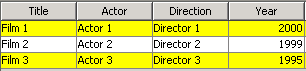
\includegraphics{PS/Table}
\caption{Table}
\label{table}
\end{center}
\end{figure}

\textbf{Mapping tables}

In the \gdomm{}, a table to be mapped looks like this:

\begin{figure}
\begin{center}
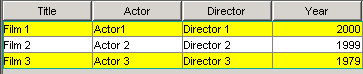
\includegraphics{PS/Maptable}
\caption{Table}
\label{maptable}
\end{center}
\end{figure}

\textbf{Virtual tables in SWT}\\
The current support for tables in \app{} has not been verified for virtual SWT tables.
